\documentclass[12pt]{article}
\usepackage{mathtools}
\usepackage{graphicx}
\usepackage{amssymb}
\usepackage{amsthm}
\usepackage{esvect}
%\hspace*{-1.5in}\noindent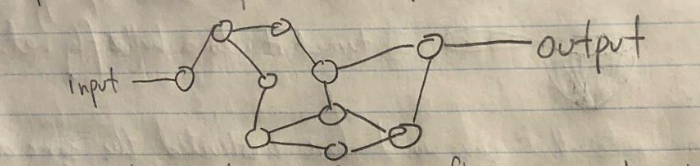
\includegraphics[scale=0.1, angle = 0]{1} \\
\graphicspath{ {./img/} }
\newcommand{\T}[0]{\mathcal{T}}
\newcommand{\B}[0]{\mathcal{B}}
\newcommand{\C}[0]{\mathcal{C}}
\newcommand{\D}[0]{\mathcal{D}}
\newcommand{\R}[0]{\mathbb{R}}
\newcommand{\Q}[0]{\mathbb{Q}}
\newcommand{\arr}[0]{\rightarrow}
\graphicspath{ {./img/} }
\begin{document}
\noindent
\textbf{Nick Franczak}\\ 
I want a system that is able to construct and review polymorphic functions.\\
A polymorphic function can evaluate to or be applied to values of different types.\\
Let $f: {A \rightarrow \B}$ be a polymorphic function where\\
${A} = \{A \in {A} \vert \text{ there is some 'structure' to A} \}$ and \\
${B} = \{B \in {A} \vert \text{ there is some 'structure' to B} \}$\\
Let $A, A^{'} \in {A}$ and $B, B^{'} \in {B}$\\
So $f(A) = B$ and $f(A^{'}) = B^{'}$\\
If this is all true then in our language $A$ is isomorphic to $A^{'}$.\\

\noindent We want the system to be able to construct polymorphic functions but that entails the prior construct of a system that is able to construct/recognize isomorphisms.\\

\noindent we have the example of the robot in the room.\\
The robot starts in the middle of the room.\\
The fourth time the robot goes forward it runs into the wall.\\

\noindent $t = 0$ $?(i_{0}) \rightarrow m_{1}?(i_{0})$\\
\noindent $t = 1$ $?(m_{1}?(i_{0})i_{1}) \rightarrow m_{2}?(m_{1}?(i_{0})i_{1})$\\
\noindent $t = 2$ $?(m_{2}?(m_{1}?(i_{0})i_{1})i_{2}) \rightarrow m_{3}?(m_{2}?(m_{1}?(i_{0})i_{1})i_{2})$\\
\noindent $t = 3$ $?(m_{3}?(m_{2}?(m_{1}?(i_{0})i_{1})i_{2})i_{3}) \rightarrow m_{4}?(m_{3}?(m_{2}?(m_{1}?(i_{0})i_{1})i_{2})i_{3})$\\
\noindent $t = 4$ $?(m_{4}?(m_{3}?(m_{2}?(m_{1}?(i_{0})i_{1})i_{2})i_{3})i_{4}) \rightarrow m_{5}?(m_{4}?(m_{3}?(m_{2}?(m_{1}?(i_{0})i_{1})i_{2})i_{3})i_{4}) $\\
\noindent $t = 5$ $?(m_{5}?(m_{4}?(m_{3}?(m_{2}?(m_{1}?(i_{0})i_{1})i_{2})i_{3})i_{4})i_{5}) \rightarrow m_{6}?(m_{5}?(m_{4}?(m_{3}?(m_{2}?(m_{1}?(i_{0})i_{1})i_{2})i_{3})i_{4})i_{5})$\\
\noindent $t = 6$ $?(m_{6}?(m_{5}?(m_{4}?(m_{3}?(m_{2}?(m_{1}?(i_{0})i_{1})i_{2})i_{3})i_{4})i_{5})i_{7}) \rightarrow m_{7}?(m_{6}?(m_{5}?(m_{4}?(m_{3}?(m_{2}?(m_{1}?(i_{0})i_{1})i_{2})i_{3})i_{4})i_{5})i_{7})$\\
\noindent $t = 7$ $?(m_{7}?(m_{6}?(m_{5}?(m_{4}?(m_{3}?(m_{2}?(m_{1}?(i_{0})i_{1})i_{2})i_{3})i_{4})i_{5})i_{7})i_{7}) \rightarrow m_{8}?(m_{7}?(m_{6}?(m_{5}?(m_{4}?(m_{3}?(m_{2}?(m_{1}?(i_{0})i_{1})i_{2})i_{3})i_{4})i_{5})i_{7})i_{7})$\\
\noindent $t = 8$ $?(m_{8}?(m_{7}?(m_{6}?(m_{5}?(m_{4}?(m_{3}?(m_{2}?(m_{1}?(i_{0})i_{1})i_{2})i_{3})i_{4})i_{5})i_{7})i_{7})i_{8}) \rightarrow m_{9}?(m_{8}?(m_{7}?(m_{6}?(m_{5}?(m_{4}?(m_{3}?(m_{2}?(m_{1}?(i_{0})i_{1})i_{2})i_{3})i_{4})i_{5})i_{7})i_{7})i_{8}) $\\
\noindent $t = 9$ $?(m_{9}?(m_{8}?(m_{7}?(m_{6}?(m_{5}?(m_{4}?(m_{3}?(m_{2}?(m_{1}?(i_{0})i_{1})i_{2})i_{3})i_{4})i_{5})i_{7})i_{7})i_{8})i_{9}) \rightarrow m_{10}?(m_{9}?(m_{8}?(m_{7}?(m_{6}?(m_{5}?(m_{4}?(m_{3}?(m_{2}?(m_{1}?(i_{0})i_{1})i_{2})i_{3})i_{4})i_{5})i_{7})i_{7})i_{8})i_{9})$\\
\noindent $t = 10$ $?(m_{10}?(m_{9}?(m_{8}?(m_{7}?(m_{6}?(m_{5}?(m_{4}?(m_{3}?(m_{2}?(m_{1}?(i_{0})i_{1})i_{2})i_{3})i_{4})i_{5})i_{7})i_{7})i_{8})i_{9})i_{10}) \rightarrow m_{11}?(m_{10}?(m_{9}?(m_{8}?(m_{7}?(m_{6}?(m_{5}?(m_{4}?(m_{3}?(m_{2}?(m_{1}?(i_{0})i_{1})i_{2})i_{3})i_{4})i_{5})i_{7})i_{7})i_{8})i_{9})i_{10})$\\
\noindent $t = 11$ $?(m_{11}?(m_{10}?(m_{9}?(m_{8}?(m_{7}?(m_{6}?(m_{5}?(m_{4}?(m_{3}?(m_{2}?(m_{1}?(i_{0})i_{1})i_{2})i_{3})i_{4})i_{5})i_{7})i_{7})i_{8})i_{9})i_{10})i_{11}) \rightarrow m_{12}?(m_{11}?(m_{10}?(m_{9}?(m_{8}?(m_{7}?(m_{6}?(m_{5}?(m_{4}?(m_{3}?(m_{2}?(m_{1}?(i_{0})i_{1})i_{2})i_{3})i_{4})i_{5})i_{7})i_{7})i_{8})i_{9})i_{10})i_{11})$\\
\noindent $t = 12$ $?() \rightarrow m_{}$\\
\noindent $t = 12$ $?() \rightarrow m_{}$\\
\noindent $t = 12$ $?() \rightarrow m_{}$\\
\noindent $t = 12$ $?() \rightarrow m_{}$\\
\noindent $t = 12$ $?() \rightarrow m_{}$\\
\noindent $t = 12$ $?() \rightarrow m_{}$\\

\noindent this is impossible to keep track of. so lets add a variable to keep track of the previous state?\\
so starting from the top we have
\begin{center}
$\underline{?(i_{0})} \rightarrow \underline{m_{1}?(i_{0})}$
\end{center}

\begin{center}
$?(m_{1}\underline{?(i_{0})}i_{1}) \rightarrow m_{2}?(\underline{m_{1}?(i_{0})}i_{1})$
\end{center}

\begin{center}
$?(m_{2}?(m_{1}\underline{?(i_{0})}i_{1})i_{2}) \rightarrow m_{3}?(m_{2}?(\underline{m_{1}?(i_{0})}i_{1})i_{2})$
\end{center}


\begin{center}
$?(m_{3}?(m_{2}?(m_{1}\underline{?(i_{0})}i_{1})i_{2})i_{3}) \rightarrow m_{4}?(m_{3}?(m_{2}?(\underline{m_{1}?(i_{0})}i_{1})i_{2})i_{3})$
\end{center}


\noindent all these are of form $a \rightarrow b$, except at each time interval, both $a$ and $b$ grow. We see that generally

\noindent look into second order logic with quantifying over predicates\\
\noindent look also into higher order logic\\
\noindent third order logic.. ?\\
w\\
w\\
w\\
w\\
w\\
w\\
w\\
w\\
w\\
w\\
w\\
w\\
w\\
w\\
w\\






-------------------------------------------------------------------------------------------\\


\noindent $t = 0$\\
$?(i) \arr m?(i)$\\
With ${\T} = \emptyset $\\

\noindent $t = 1$\\
$?(m?(i)w) \arr m?(m?(i)w)$\\
With ${\T} = \{mi \arr w \}$\\

\noindent $t = 2$\\
$?(m?(m?(i)w)w) \arr m?(m?(m?(i)w)w)$\\
With ${\T} = \{ \{mi \arr w\} , \{mw \arr w\} \}$\\

\noindent $t = 3$\\
$?(m?(m?(m?(i)w)w)w) \arr m^{-1}?(m?(m?(m?(i)w)w)w)$\\
With ${\T} = \{ \{mi \arr w\} , \{mw \arr w\}, \{mw \arr w\} \}$\\
This implies 
With ${\T} = \{ \{mi \arr w\} , \{m\forall w \arr w\}\}$\\

\noindent For brevity let $m?(m?(m?(i)w)w)w = \alpha$\\

\noindent $t = 4$\\
$?(m^{-1}?(\alpha)i) \arr m^{-1}?(m^{-1}?(\alpha)i) $\\
With ${\T} = \{ \{mi \arr w\} , \{mw \arr w\}, \{mw \arr w\} \}$\\
This implies 
With ${\T} = \{ \{mi \arr w\} , \{m\forall w \arr w\}\}$\\








\end{document}